\documentclass[letterpaper]{scrartcl}
\usepackage{lmodern}
\usepackage{amssymb,amsmath}
\usepackage{ifxetex,ifluatex}
\usepackage{fixltx2e} % provides \textsubscript
\ifnum 0\ifxetex 1\fi\ifluatex 1\fi=0 % if pdftex
  \usepackage[T1]{fontenc}
  \usepackage[utf8]{inputenc}
\else % if luatex or xelatex
  \ifxetex
    \usepackage{mathspec}
    \usepackage{xltxtra,xunicode}
  \else
    \usepackage{fontspec}
  \fi
  \defaultfontfeatures{Mapping=tex-text,Scale=MatchLowercase}
  \newcommand{\euro}{€}
\fi
% use upquote if available, for straight quotes in verbatim environments
\IfFileExists{upquote.sty}{\usepackage{upquote}}{}
% use microtype if available
\IfFileExists{microtype.sty}{%
\usepackage{microtype}
\UseMicrotypeSet[protrusion]{basicmath} % disable protrusion for tt fonts
}{}
\usepackage[margin=1in]{geometry}
\usepackage{graphicx}
\makeatletter
\def\maxwidth{\ifdim\Gin@nat@width>\linewidth\linewidth\else\Gin@nat@width\fi}
\def\maxheight{\ifdim\Gin@nat@height>\textheight\textheight\else\Gin@nat@height\fi}
\makeatother
% Scale images if necessary, so that they will not overflow the page
% margins by default, and it is still possible to overwrite the defaults
% using explicit options in \includegraphics[width, height, ...]{}
\setkeys{Gin}{width=\maxwidth,height=\maxheight,keepaspectratio}
\ifxetex
  \usepackage[setpagesize=false, % page size defined by xetex
              unicode=false, % unicode breaks when used with xetex
              xetex]{hyperref}
\else
  \usepackage[unicode=true]{hyperref}
\fi
\hypersetup{breaklinks=true,
            bookmarks=true,
            pdfauthor={Gus Dunn},
            pdftitle={Gloria-Soria (ddRAD58)},
            colorlinks=true,
            citecolor=blue,
            urlcolor=blue,
            linkcolor=magenta,
            pdfborder={0 0 0}}
\urlstyle{same}  % don't use monospace font for urls
\setlength{\parindent}{0pt}
\setlength{\parskip}{6pt plus 2pt minus 1pt}
\setlength{\emergencystretch}{3em}  % prevent overfull lines
\setcounter{secnumdepth}{5}

\title{Gloria-Soria (ddRAD58)}
\author{Gus Dunn}
\date{2014-12-29}
\usepackage{fontspec}
\setmainfont{Linux Libertine O}

% blockquote


\begin{document}
\maketitle

{
\hypersetup{linkcolor=black}
\setcounter{tocdepth}{3}
\tableofcontents
}
\section{Functional Annotations}\label{functional-annotations}

\subsection{Sequences Used}\label{sequences-used}

\textbf{\emph{Glossina fuscipes fuscipes:}} All putative peptides
annotated for \emph{G. f. fuscipes} in the GfusI1.1 gene-build were
obtained from \href{link_address}{VectorBase} {[}1{]}

\textbf{Other:} The sequences used to compare the \emph{G. f. fuscipes}
peptides against well known/annotated sequences were obtained from
UNIPROT/SwissProt {[}2{]}~(used with \texttt{blastp}) and PFAM
{[}3{]}~(used with \texttt{hmmscan}) as required by
\href{link_address}{ARGOT2} {[}4--6{]}.

\subsection{Argot2 Analysis}\label{argot2-analysis}

The \texttt{blastp} and \texttt{hmmscan} results submitted to ARGOT2
were obtained by performing local searches on the \emph{G. f. fuscipes}
peptides against the UNIPROT peptide database (obtained on 2014-09-08)
and the hidden Markov models (HMM) of the combined protein-domain sets
om the Pfam databases (Pfam-A and Pfam-B: obtained on 2014-09-08),
respectively. Settings used were as dictated by the ARGOT2 site.

The \texttt{blastp} and \texttt{hmmscan} results were uploaded to ARGOT2
servers for analysis after being split into 10 groups (roughly 2330
peptides per group) to prevent overloading the remote ARGOT2 cluster.
The functional annotations were then downloaded and joined back
together.

\section{Linkage Analysis}\label{linkage-analysis}

\subsection{Source of SNPs}\label{source-of-snps}

SNPs were obtained as described earlier in this manuscript.

\subsection{Linkage measurements}\label{linkage-measurements}

Plink version 1.9 {[}7{]} was used to calculate pairwise linkage
disequilibrium (LD) as \(r\) for all SNP-pairs located on common
supercontigs. The \texttt{-\/-allow-extra-chr} option was required to
handle the number of supercontigs. Unless stated otherwise, all
subsequent analysis pertaining to LD used \(r^2\).

\subsection{LD-based filtering of
SNP-pairs}\label{ld-based-filtering-of-snp-pairs}

The LD values of SNP-pairs were compared after binning SNP-pairs by base
pair separation to control for unknown rates of recombination in
\emph{G. f. fuscipes}. Bin length was set at 50 bp with the lower bound
inclusive and higher bound exclusive. In other words the bins were
defined as \([i, i + 49)\) where
\(i \in \{1,1(50),2(50),3(50) ... n(50)\}\) and \(n\) is a positive
integer.

To identify SNP-pairs for further investigation in an arbitrary set of
binned SNP-pairs, we needed to assign probabilities to each SNP-pair in
the bin. The distributions of binned SNP-pairs are bounded by 0 and 1
and do not appear to be Normal in shape. Additionally, in many cases,
the data appear to exhibit peaks at both the lower and upper \(r^2\)
range. This suggested that the data may be modeled well using the
probability density function (PDF) of the Beta distribution:

\[f(x;\alpha,\beta) = \frac{x^{\alpha-1}(1-x)^{\beta-1}} {\mathrm{B}(\alpha,\beta)}\]

with shape parameters \(\alpha\) and \(\beta\) and where \(x\)
represents an observed value generated by the distribution and
\(\mathrm{B}()\) is the Beta function \textbf{\{\{CITE\_ME\}\}}.

The Beta's cumulative distribution function (CDF)

\[F(x;\alpha,\beta) = \frac{\mathrm{B}(x;\alpha,\beta)}{\mathrm{B}(\alpha,\beta)} \]

can be used to describe the probability that a binned SNP-pair will be
observed to have an \(r^2 \le x\). It follows that \(1-\mathrm{CDF}\)
represents the probability of observing a more extreme value.

For each set of binned \(r^2\) values, the SNP-pairs deemed worthy of
further investigation were defined as those where
\(1-\mathrm{CDF} \le 0.01\) after Benjamini-Hochberg (BH) correction for
multiple testing {[}8{]}.

\subsubsection{Scaling of binned \(r^2\)
distributions}\label{scaling-of-binned-r2-distributions}

The Beta distribution is bounded on the non-inclusive interval between 0
and 1. However, there are data in each bin that may have been assigned
values of exactly 0 or 1. It is likely that these values are not truly 0
or 1 in the discrete binary since that a coin-flip is \emph{either}
heads or tails. Therefore, the all data for each bin were scaled
according to the following scheme

\[((x_i - 0.5)\cdot \theta) + 0.5\]

in order to symmetrically shrink the distribution of values to fit
within the open interval \((0,1)\). In the scheme above, let \(x_i\)
stand for the \(r^2\) of each SNP-pair in an arbitrary bin set and
\(\theta\) stand for the scaling factor. The relevant results in this
paper used \(\theta = 0.999\).

\subsubsection{Bayesian parameter estimation using the binned \(r^2\)
distributions}\label{bayesian-parameter-estimation-using-the-binned-r2-distributions}

In order to use the CDF of the Beta distribution to assign significances
to each observed SNP-pair in a bin, it is necessary to learn the
distribution parameters (\(\alpha\) and \(\beta\)) for each bin given
the specific data in each bin. For this we used custom python code that
made heavy use of the following third-party data analysis modules:
Pandas {[}9{]}, NumPy {[}10{]}, SciPy {[}11{]}, pyMC {[}12{]}, and
StatsModels {[}13{]}.

We used pyMC to build the model of the Beta distribution and use it to
exploit the bin-specific data to estimate the bin-specific values for
the \(\alpha\) and \(\beta\) parameters of the model {[}Figure
fig\_betamod{]}. The values of \(\alpha\) and \(\beta\) were modeled
with separate Uniform prior distributions from 0.01 to 10. This model
topology was used to create pyMC ``model'' objects and initialized with
the \(r^2\) data from each bin. The parameters of each Beta distribution
were then estimated by \emph{maximum a posteriori} (MAP) and used to
calculate the \(1-\mathrm{CDF}\) for each SNP-pair in each bin
{[}10,11{]}. The \(1-\mathrm{CDF}\) values were then BH corrected by bin
and filtered with a threshold of \((1-CDF)_{BH} \le 0.01\) using
statsmodels {[}8{]}.

\hyperdef{}{figux5fbetamod}{}
\begin{figure}[htbp]
\centering
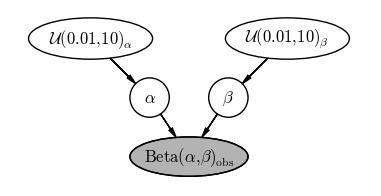
\includegraphics{../figures/bin_MAP_model.png}
\caption{\textbf{{[}fig\_betamod{]}Network representation of the LD Beta
model:} Ovals represent modeled probability distributions. Circles
represent learned parameters. Grey shading indicates use of observed
data. \label{fig_betamod}}
\end{figure}

\newpage

\section*{Bibliography}\label{bibliography}
\addcontentsline{toc}{section}{Bibliography}

1. Giraldo-Calderon GI, Emrich SJ, MacCallum RM, Maslen G, Dialynas E,
Topalis P, et al. VectorBase: an updated bioinformatics resource for
invertebrate vectors and other organisms related with human diseases.
Nucleic Acids Research. 2014;43: D707--D713.
doi:\href{http://dx.doi.org/10.1093/nar/gku1117}{10.1093/nar/gku1117}

2. Boeckmann B, Blatter M-C, Famiglietti L, Hinz U, Lane L, Roechert B,
et al. Protein variety and functional diversity: Swiss-Prot annotation
in its biological context. Comptes rendus biologies. 2005;328: 882--99.
doi:\href{http://dx.doi.org/10.1016/j.crvi.2005.06.001}{10.1016/j.crvi.2005.06.001}

3. Finn RD, Bateman A, Clements J, Coggill P, Eberhardt RY, Eddy SR, et
al. Pfam: the protein families database. Nucleic acids research.
2014;42: D222--30.
doi:\href{http://dx.doi.org/10.1093/nar/gkt1223}{10.1093/nar/gkt1223}

4. Radivojac P, Clark WT, Oron TR, Schnoes AM, Wittkop T, Sokolov A, et
al. A large-scale evaluation of computational protein function
prediction. Nature methods. Nature Publishing Group, a division of
Macmillan Publishers Limited. All Rights Reserved. 2013;10: 221--7.
doi:\href{http://dx.doi.org/10.1038/nmeth.2340}{10.1038/nmeth.2340}

5. Falda M, Toppo S, Pescarolo A, Lavezzo E, {Di Camillo} B, Facchinetti
A, et al. Argot2: a large scale function prediction tool relying on
semantic similarity of weighted Gene Ontology terms. BMC bioinformatics.
BioMed Central Ltd; 2012;13 Suppl 4: S14.
doi:\href{http://dx.doi.org/10.1186/1471-2105-13-S4-S14}{10.1186/1471-2105-13-S4-S14}

6. Gillis J, Pavlidis P. Characterizing the state of the art in the
computational assignment of gene function: lessons from the first
critical assessment of functional annotation (CAFA). BMC Bioinformatics.
BioMed Central Ltd; 2013;14: S15.
doi:\href{http://dx.doi.org/10.1186/1471-2105-14-S3-S15}{10.1186/1471-2105-14-S3-S15}

7. Chang CC, Chow CC, Tellier LC, Vattikuti S, Purcell SM, Lee JJ.
Second-generation PLINK: rising to the challenge of larger and richer
datasets. GigaScience. BioMed Central Ltd; 2015;4: 7.
doi:\href{http://dx.doi.org/10.1186/s13742-015-0047-8}{10.1186/s13742-015-0047-8}

8. Benjamini Y, Hochberg Y. Controlling the False Discovery Rate: A
Practical and Powerful Approach to Multiple Testing. Journal of the
Royal Statistical Society Series B (Methodological). Wiley for the Royal
Statistical Society; 1995;57: pp. 289--300. Available:
\url{http://www.jstor.org/stable/2346101}

9. McKinney W. Data Structures for Statistical Computing in Python. In:
Walt S van der, Millman J, editors. Proceedings of the 9th python in
science conference. 2010. pp. 51--56.

10. {Van Der Walt} S, Colbert SC, Varoquaux G. The NumPy array: A
structure for efficient numerical computation. Computing in Science and
Engineering. 2011;13: 22--30.
doi:\href{http://dx.doi.org/10.1109/MCSE.2011.37}{10.1109/MCSE.2011.37}

11. Jones E, Oliphant T, Peterson P, Others. SciPy: Open source
scientific tools for Python {[}Internet{]}. 2001. Available:
\url{http://www.scipy.org/}

12. Patil A, Huard D, Fonnesbeck CJ. PyMC: Bayesian Stochastic Modelling
in Python. Journal of statistical software. 2010;35: 1--81. Available:
\url{http://www.pubmedcentral.nih.gov/articlerender.fcgi?artid=3097064/\&tool=pmcentrez/\&rendertype=abstract}

13. Statsmodels-development-team. StatsModels: Statistics in Python
(v0.6.1) {[}Internet{]}. Available:
\url{http://statsmodels.sourceforge.net/stable/}

\end{document}
